\chapter{Ideen und Konzepte}

Im folgenden Kapitel wird auf die grundlegenden Architekturentscheidungen
eingegangen und erklährt wieso diese so umgesetzt wurden.

\section{Architektur}

Da die Applikation laut dem Auftraggeber skalierbar sein sollte, wurde
eine Mikroservice Architektur in Betracht gezogen.

Bei einer solchen Architektur werden die einzelnen unabhängigen Komponenten
einer Software\footnote{
    In diesem fall könnte das beispielsweise die Datenverarbeitung via MQTT
    von den \ac{IoT} Geräten und das Web Frontend sein.
} in verschiedene kleinere Komponenten unterteilt.
Diese Komponenten können danach unabhängig voneinander entwickelt und
releast werden.
Die Kommunikation zwischen den einzelnen Komponenten geschieht mittels
vordeffinierter \ac{API}s. Häuffig werden Message Queues wie RabbitMQ dafür
eingesetzt. Wichtig dabei ist auch dass die Datenschemen der einzelnen
Microservices unabhängig voneinander sind. Das heisst, jeder Microservice
besitzt eine eigene Datenbank. \cite{microservices}
Um die einzelnen Komponenten danach unabhängig voneinander releasen zu
können, werden häufig Container basierte Deployments verwendet.\footnote{
    Wie beispielsweise Docker oder Podman.
}
Diese Deployments werden danach meist auf einen Orchestrator wie Kubernetes
deployt.

In dieser Arbeit wird keine Microservice Architektur im klassischen Sinne verwendet.
Die einzelnen Komponenten werden zwar in sepparate Container deployt (Abbildung: \ref{fig:smic-arch})
besitzen jedoch keine eigene Datenbank.
Das hat den Vorteil, dass weniger Overhead implementiert werden muss (mittels Message Queue)
und das Datenbankschema kann zentral in der Datastore Python library einmal implementiert
und dann in den verschiedenen Komponenten wiederverwendet werden.


\begin{figure}[h]
    \centering
    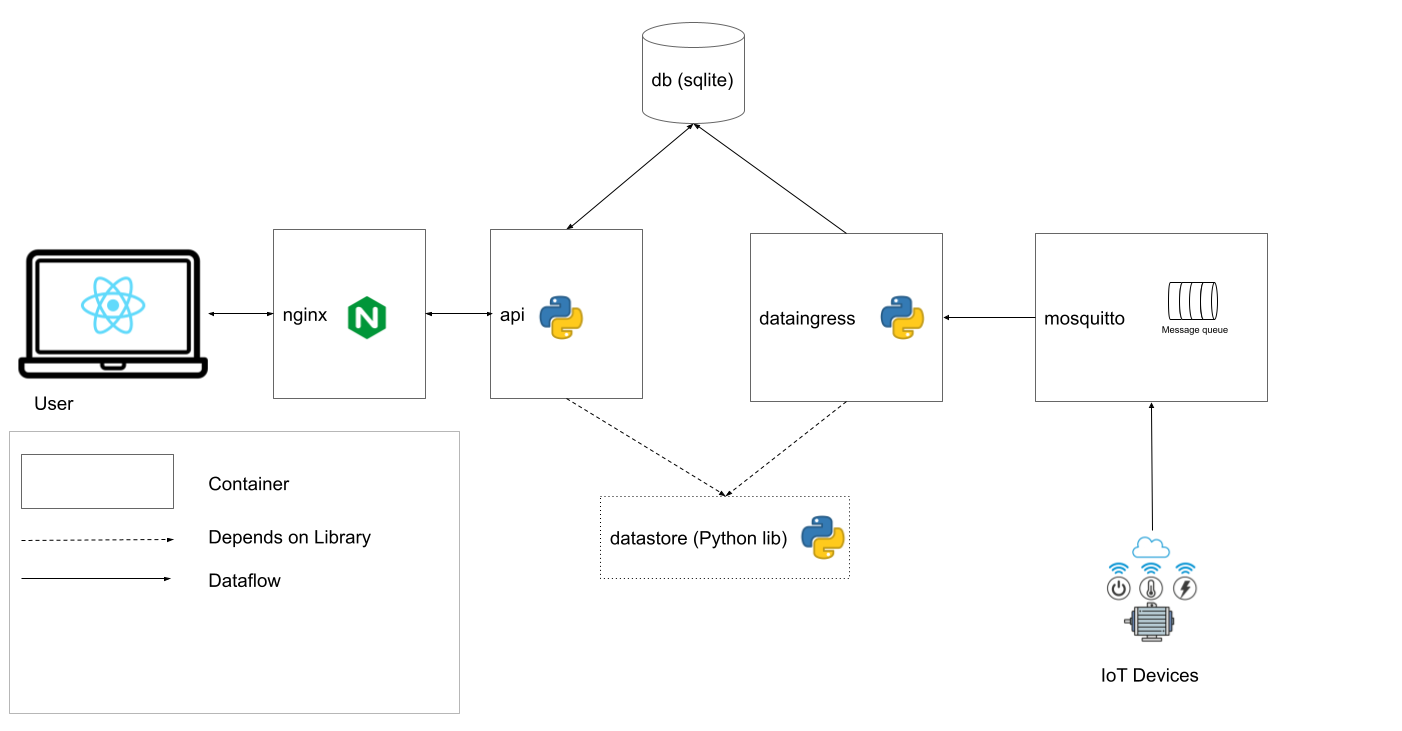
\includegraphics[width=1.0\textwidth]{gfx/smic-arch}
    \caption{
        Schamatische Darstellung der in diesem Projekt verwendeten Architektur
    }
    \label{fig:smic-arch}
\end{figure}

Die Abbildung \ref{fig:smic-arch} zeigt die in diesem Projekt verwendete
Architektur auf. Hier noch einige Informationen zu den einzelnen Komponenten:


\begin{itemize}
    \item \texttt{nginx}:
        Alle Anfragen des Endbenutzer werden über einen Nginx Server
        engegengenommen. Dieser liefert dann dem Benutzer die React WebApp
        oder leitet Anfragen an die \ac{API} weiter.

    \item \texttt{api}:
        Die \ac{API} verarbeitet Datenanfragen der React WebApp. Sie gibt
        beispielsweise die Stromzählerdaten eines Tages zurück.

    \item \texttt{datastore}:
        Der datastore ist eine Python library, die das Datenbankschema festlegt.
        Sowohl die \ac{API} als auch der dataingress greiffen auf die Datenbank zu
        und verwenden somit die datastore library.

    \item \texttt{dataingress}:
        Der dataingress arbeitet die von den \ac{IoT} geräten gesendeten
        Stromzählerdaten ab und speichert diese in die Datenbank.

    \item \texttt{mosquitto}:
        Mosquitto ist der in dieser Arbeit verwendete \ac{MQTT} Broker.
\end{itemize}

Ein weiterer grund für die Entscheidung einer geteilten Datenbank ist,
dass der \texttt{dataingress} keine Daten liest sondern diese nur von
der \ac{MQTT} Queue abarbeitet und in die Datenbank schreibt.